\section{Experimentos y resultados}
\label{sec:resultados}

\textbf{Protocolo (entregable 3).} La métrica principal es la oficial: AUC-ROC macro sobre las
doce etiquetas en los 58 dorados. Los IC 95\,\% se obtienen por bootstrap de estudios (1\,000
remuestreos), y las diferencias entre corridas, con un bootstrap pareado: los mismos
remuestreos para ambas corridas. Precisión, recall y F1 se reportan al umbral elegido en
\texttt{weak\_val}. Ese umbral se justifica porque no toca los dorados, pero hereda el cambio
de prevalencia entre la muestra y los dorados (Sección~\ref{sec:datos}). Incluimos dos
referencias: un predictor constante (AUC 0,5) y el propio extractor de texto, que lee el
reporte en lugar de la imagen.

\begin{table}[t]
  \caption{Resultados en los 58 dorados. AUC macro con IC 95\,\% por bootstrap; \emph{56}:
    sin los dos dorados de serie de respaldo; P/R/F1 macro al umbral elegido en
    \texttt{weak\_val}. B: media $\pm$ desviación estándar de tres semillas en la última fila.}
  \label{tab:main}
  \centering
  \small
  \begin{tabular}{lcccccc}
    \toprule
    Modelo & AUC macro [IC 95\,\%] & AUC (56) & P & R & F1 \\
    \midrule
    Predictor constante (prevalencia)   & 0,500 & 0,500 & -- & -- & -- \\
    Extractor de texto (lee el reporte) & 0,812 [0,777--0,847] & 0,813 & -- & -- & -- \\
    \midrule
    A: CNN desde cero                   & 0,654 [0,592--0,710] & 0,661 & 0,37 & 0,64 & 0,44 \\
    B: ResNet-50, v1 (colapsó)          & 0,649 [0,597--0,697] & 0,650 & 0,44 & 0,57 & 0,46 \\
    B: ResNet-50                        & \textbf{0,715} [0,656--0,771] & 0,722 & 0,48 & 0,61 & 0,51 \\
    B: ResNet-50, 3 semillas            & 0,716 $\pm$ 0,005 & -- & 0,53 & 0,57 & 0,50 \\
    \bottomrule
  \end{tabular}
\end{table}

\textbf{A frente a B (entregable 2).} B alcanza una AUC macro de 0,715 y supera a A, con una
diferencia pareada de $-0{,}062$ $[-0{,}114;\,-0{,}008]$ (Tabla~\ref{tab:main}). La variación
entre semillas de B es pequeña ($\pm0{,}005$), así que la diferencia no se debe al azar.

La Figura~\ref{fig:curvas}b explica la brecha. A está subajustado: tras 60 épocas, su AUC sobre
datos de entrenamiento es apenas 0,72, de modo que 510 estudios con 19\,\% de ruido no
bastan para aprender características visuales desde cero. B, en cambio, alcanza su mejor
validación hacia la época 9 (AUC de entrenamiento $\approx0{,}93$) y después empieza a
memorizar el ruido: el entrenamiento sube a 0,98 mientras la validación baja. Es el patrón
descrito por \citet{arpit2017closer}, y todas las corridas de B lo repiten entre las épocas 8
y 12, por lo que la parada temprana resulta imprescindible.

La primera versión de B (v1), que reentrenaba toda la red con tasa $10^{-4}$, colapsó al
descongelar (Figura~\ref{fig:curvas}a). Su pérdida quedó en 1,09, el valor de un predictor
constante (1,0896). La ablación \texttt{B\_all} confirma que el problema era la tasa de
aprendizaje y no la profundidad: reentrenar toda la red con $2\times10^{-5}$ da el mismo
resultado que reentrenar solo \texttt{layer3} y \texttt{layer4}.

\begin{figure}[t]
  \centering
  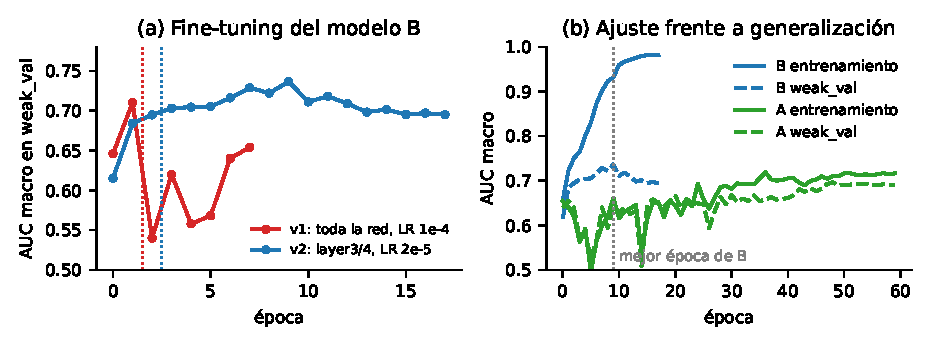
\includegraphics[width=\linewidth]{figures/curves.pdf}
  \caption{(a) Ajuste fino de B: con tasa $10^{-4}$ sobre toda la red, la AUC en
    \texttt{weak\_val} cae al descongelar (línea punteada); con $2\times10^{-5}$ sobre
    \texttt{layer3}/\texttt{layer4} sigue mejorando. (b) AUC en un subconjunto fijo de
    entrenamiento (línea continua) y en \texttt{weak\_val} (línea discontinua): B memoriza
    el ruido después de su mejor época; A no llega a ajustar ni el entrenamiento.}
  \label{fig:curvas}
\end{figure}

\textbf{Por hallazgo.} B obtiene su mejor AUC en derrame (0,89), artrosis medial (0,84) y
contusión (0,76), y la peor en meniscos (0,60--0,64); ver la Tabla~\ref{tab:perlabel}.

En tres hallazgos B \emph{supera al extractor de texto con el que se entrenó}: derrame (0,89
frente a 0,68), artrosis medial (0,84 frente a 0,80) y sinovitis (0,68 frente a 0,64). Son los hallazgos que el reporte tiende a omitir ($\kappa\approx0{,}3$ en la
Tabla~\ref{tab:etiquetas}). La red recupera el patrón visual a pesar de las etiquetas
ruidosas, lo que es coherente con que los dorados se hayan anotado sobre la imagen. En promedio,
sin embargo, el texto sigue arriba: $+0{,}096$ $[0{,}036;\,0{,}157]$.

\begin{table}[t]
  \caption{AUC por hallazgo en los dorados: A, B (sagital), B con la vista coronal y el
    extractor de texto como referencia.}
  \label{tab:perlabel}
  \centering
  \footnotesize
  \setlength{\tabcolsep}{2.3pt}
  \begin{tabular}{lcccccccccccc|c}
    \toprule
    & LCA & LCM & M.\,med. & M.\,lat. & A.\,med. & A.\,lat. & A.\,PF & Derr. & Sinov. & Baker & Cont. & Fract. & Macro \\
    \midrule
    A             & 0,67 & 0,39 & 0,58 & \textbf{0,76} & 0,74 & 0,67 & 0,69 & 0,81 & \textbf{0,69} & 0,64 & 0,64 & 0,57 & 0,654 \\
    B             & \textbf{0,71} & \textbf{0,71} & 0,60 & 0,64 & 0,84 & 0,70 & 0,70 & \textbf{0,89} & 0,68 & 0,65 & \textbf{0,76} & 0,70 & 0,715 \\
    B coronal     & 0,63 & 0,57 & \textbf{0,67} & 0,63 & \textbf{0,94} & \textbf{0,74} & \textbf{0,77} & \textbf{0,89} & 0,65 & \textbf{0,92} & 0,75 & \textbf{0,82} & \textbf{0,749} \\
    \midrule
    Texto         & 0,96 & 0,93 & 0,87 & 0,88 & 0,80 & 0,71 & 0,80 & 0,68 & 0,64 & 0,91 & 0,76 & 0,81 & 0,812 \\
    \bottomrule
  \end{tabular}
\end{table}

\textbf{Ablaciones (entregable 4).} Cada corrida cambia un solo factor respecto de B
(Tabla~\ref{tab:ablacion}). Con 58 dorados y una variación entre semillas de $\pm0{,}01$, solo
una diferencia resulta concluyente: \textbf{entrenar únicamente con etiquetas de alta
confianza empeora el modelo} ($-0{,}044$ $[-0{,}087;\,-0{,}005]$). Descartar las etiquetas
dudosas elimina más supervisión útil que ruido.

Ponderar por confianza y usar la pérdida focal no cambian la AUC. La vista coronal obtiene el
mejor valor (0,749), aunque sin significancia ($+0{,}034$ $[-0{,}016;\,0{,}081]$). Las dos vistas
son complementarias:
\begin{itemize}
  \item la coronal es mejor en quiste de Baker (0,92 frente a 0,65), fractura (0,82 frente a
        0,70) y artrosis medial (0,94 frente a 0,84);
  \item la sagital es mejor en el LCA y el LCM.
\end{itemize}
Esto sugiere que fusionar ambas vistas es la mejora más prometedora.

\begin{table}[t]
  \caption{Ablaciones sobre B: diferencia de AUC macro con IC 95\,\% por bootstrap pareado.
    En negrita, la única diferencia cuyo IC excluye el cero.}
  \label{tab:ablacion}
  \centering
  \small
  \begin{tabular}{llccc}
    \toprule
    Factor & Variante frente a B & AUC macro & $\Delta$ [IC 95\,\%] & F1 macro \\
    \midrule
    Semilla       & semilla 1 / semilla 2 & 0,722 / 0,712 & +0,006 / $-$0,004 & 0,53 / 0,47 \\
    Pérdida       & focal ($\gamma=2$) & 0,722 & +0,007 [$-$0,025; 0,035] & 0,52 \\
    Ruido         & ponderar por confianza & 0,713 & $-$0,003 [$-$0,026; 0,016] & 0,49 \\
    Ruido         & solo alta confianza & \textbf{0,672} & \textbf{$-$0,044 [$-$0,087; $-$0,005]} & 0,47 \\
    Desbalance    & sin \texttt{pos\_weight} & 0,718 & +0,003 [$-$0,034; 0,037] & 0,49 \\
    Profundidad   & reentrenar toda la ResNet & 0,718 & +0,003 [$-$0,024; 0,027] & 0,51 \\
    Plano         & coronal & 0,749 & +0,034 [$-$0,016; 0,081] & 0,52 \\
    \bottomrule
  \end{tabular}
\end{table}

\textbf{Mitigación del desbalance (entregable 6).} \texttt{pos\_weight} no cambia la AUC
(0,715 frente a 0,718 sin él). Es lo esperable: la AUC solo mide el orden de las predicciones,
y el peso actúa sobre la calibración. El efecto se ve en el recall de los hallazgos raros al
umbral elegido, pero es mixto:
\begin{itemize}
  \item contusión: 0,79 con el peso y 0,05 sin él;
  \item fractura: 0,67 con el peso y 0,83 sin él.
\end{itemize}
Además es del mismo tamaño que la variación entre semillas (contusión: de 0,21 a 0,79),
porque el umbral se elige con apenas 9 o 10 positivos en \texttt{weak\_val}. La pérdida focal
tampoco mejora el recall de los raros. Concluimos que, con esta validación, la mitigación
implementada no tiene un efecto distinguible del azar, y que el cuello de botella para los
hallazgos raros es el umbral, no la pérdida.
